% Source-coordinate reconstruction. Edit named defaults or copy this entire composition.
\studiodeclarefield{graphic-1}{
\includegraphics[width=1691\studiounit]{images/studio/collection/figma-0915-part-01.pdf}}
\studiodeclarefield{graphic-2}{
\includegraphics[width=322\studiounit]{images/studio/collection/figma-0915-part-02.pdf}}
\studiodeclarefield{graphic-3}{
\includegraphics[width=321\studiounit]{images/studio/collection/figma-0915-part-03.pdf}}
\studiodeclarefield{graphic-4}{
\includegraphics[width=88\studiounit]{images/studio/collection/figma-0915-part-04.pdf}}
\studiodeclarefield{graphic-5}{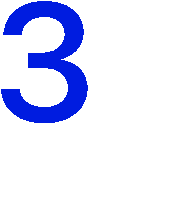
\includegraphics[width=90\studiounit]{images/studio/collection/figma-0915-part-05.pdf}}
\studiodeclarefield{title}{Payment Channels}
\studiodeclarefield{text-2}{A payment channel is a\\financial relationship\\between two nodes, which,\\through a smart contract,\\are able to make payments\\to each other without\\having to record every\\transaction on the Bitcoin\\blockchain.\par Only the opening and\\closing transactions are\\saved on-chain.}
\studiodeclarefield{text-3}{0.123}
\studiodeclarefield{text-4}{0.0005}
\studiodeclarefield{text-5}{0.03}
\studiodeclarefield{text-6}{0.0004}
\studiodeclarefield{text-7}{0.09}
\studiodeclarefield{text-8}{0.00007}
\studioapplyfields
\studiomeasuredcanvas{3556}{2000}{payment-channel}{studio-paper}{
\studiographfield{graphic-1}{1571}{277}{1691}{316}{}{}
\path[fill=studio-paper,draw=none,line width=1\studiounit,rounded corners=0\studiounit] (1766,412) rectangle (1918,453);
\path[fill=studio-paper,draw=none,line width=1\studiounit,rounded corners=0\studiounit] (2043,412) rectangle (2195,453);
\path[fill=studio-paper,draw=none,line width=1\studiounit,rounded corners=0\studiounit] (2322,412) rectangle (2474,453);
\path[fill=studio-paper,draw=none,line width=1\studiounit,rounded corners=0\studiounit] (2875,412) rectangle (3027,453);
\path[fill=studio-paper,draw=none,line width=1\studiounit,rounded corners=0\studiounit] (2595,412) rectangle (2747,453);
\studiomeasuredtext{title}{257.441}{417.984}{1055.55}{168.645}{112.735}{130.772}{\color{bitpolito}\bfseries}{\studiofield{title}}
\studiomeasuredtext{text-2}{250.648}{613.277}{871.435}{1011.61}{65.76}{76.2816}{\color{bitpolito}}{\studiofield{text-2}}
\studiographfield{graphic-2}{1841}{884}{322}{322}{}{}
\studiographfield{graphic-3}{2678}{884}{321}{322}{}{}
\path[fill=bitpolito,draw=none,line width=1\studiounit] (2566.5,969)--(2566.5,961.5)--(2159,961.5)--(2159,969)--(2159,976.5)--(2566.5,976.5)--(2566.5,969)--cycle (2634,969)--(2559,925.699)--(2559,1012.3)--(2634,969)--cycle;
\path[fill=bitpolito,draw=none,line width=1\studiounit] (2226.5,1075.99)--(2226.5,1083.49)--(2634,1083.49)--(2634,1075.99)--(2634,1068.49)--(2226.5,1068.49)--(2226.5,1075.99)--cycle (2159,1075.99)--(2234,1119.29)--(2234,1032.69)--(2159,1075.99)--cycle;
\path[fill=bitpolito,draw=none,line width=1\studiounit] (2809,622.5)--(2801.5,622.5)--(2801.5,865)--(2809,865)--(2816.5,865)--(2816.5,622.5)--(2809,622.5)--cycle (2809,555)--(2765.7,630)--(2852.3,630)--(2809,555)--cycle;
\path[fill=bitpolito,draw=none,line width=1\studiounit] (1978,622.5)--(1970.5,622.5)--(1970.5,865)--(1978,865)--(1985.5,865)--(1985.5,622.5)--(1978,622.5)--cycle (1978,555)--(1934.7,630)--(2021.3,630)--(1978,555)--cycle;
\path[fill=bitpolito,draw=none,line width=1\studiounit] (2627,1732)--(2627,1727)--(2212,1727)--(2212,1732)--(2212,1737)--(2627,1737)--(2627,1732)--cycle (2167,1732)--(2217,1760.87)--(2217,1703.13)--(2167,1732)--cycle;
\path[fill=bitpolito,draw=none,line width=1\studiounit] (2627,1380)--(2627,1375)--(2212,1375)--(2212,1380)--(2212,1385)--(2627,1385)--(2627,1380)--cycle (2167,1380)--(2217,1408.87)--(2217,1351.13)--(2167,1380)--cycle;
\path[fill=bitpolito,draw=none,line width=1\studiounit] (2627,1556)--(2627,1551)--(2212,1551)--(2212,1556)--(2212,1561)--(2627,1561)--(2627,1556)--cycle (2167,1556)--(2217,1584.87)--(2217,1527.13)--(2167,1556)--cycle;
\path[fill=bitpolito,draw=none,line width=1\studiounit] (2167,1468)--(2167,1473)--(2582,1473)--(2582,1468)--(2582,1463)--(2167,1463)--(2167,1468)--cycle (2627,1468)--(2577,1439.13)--(2577,1496.87)--(2627,1468)--cycle;
\path[fill=bitpolito,draw=none,line width=1\studiounit] (2167,1820)--(2167,1825)--(2582,1825)--(2582,1820)--(2582,1815)--(2167,1815)--(2167,1820)--cycle (2627,1820)--(2577,1791.13)--(2577,1848.87)--(2627,1820)--cycle;
\path[fill=bitpolito,draw=none,line width=1\studiounit] (2167,1644)--(2167,1649)--(2582,1649)--(2582,1644)--(2582,1639)--(2167,1639)--(2167,1644)--cycle (2627,1644)--(2577,1615.13)--(2577,1672.87)--(2627,1644)--cycle;
\path[fill=bitpolito,draw=none,line width=1\studiounit] (1661.85,1045)--(1661.85,997.344)--(1661.66,997.344)--(1646.93,1007.5)--(1646.93,999.18)--(1661.77,988.633)--(1670.45,988.633)--(1670.45,1045)--(1661.85,1045)--cycle;
\studiographfield{graphic-4}{2076}{1350}{88}{106}{}{}
\studiographfield{graphic-5}{2677}{680}{90}{107}{}{}
\studiomeasuredtext{text-3}{2348.24}{1321.92}{124.744}{52.984}{40.76}{47.2816}{\color{bitpolito}}{\studiofield{text-3}}
\studiomeasuredtext{text-4}{2330.09}{1415.92}{161.705}{52.984}{40.76}{47.2816}{\color{bitpolito}}{\studiofield{text-4}}
\studiomeasuredtext{text-5}{2356.18}{1499.92}{108.873}{52.984}{40.76}{47.2816}{\color{bitpolito}}{\studiofield{text-5}}
\studiomeasuredtext{text-6}{2329.12}{1590.92}{162.892}{52.984}{40.76}{47.2816}{\color{bitpolito}}{\studiofield{text-6}}
\studiomeasuredtext{text-7}{2355.16}{1672.92}{110.193}{52.984}{40.76}{47.2816}{\color{bitpolito}}{\studiofield{text-7}}
\studiomeasuredtext{text-8}{2318.22}{1766.92}{185.115}{52.984}{40.76}{47.2816}{\color{bitpolito}}{\studiofield{text-8}}
}
